\documentclass[11pt]{article}

\usepackage{epsfig}
\usepackage{amsfonts}
\usepackage{amssymb}
\usepackage{amstext}
\usepackage{amsmath}
\usepackage{xspace}
\usepackage{theorem}
\usepackage{hyperref}
\usepackage{fullpage}
\usepackage{framed}

\usepackage{enumitem}                     
\usepackage{listings}
\usepackage{color}

\usepackage{titlesec}

\usepackage{tikz}
\usepackage{graphicx}
\usetikzlibrary{positioning}

\definecolor{dkgreen}{rgb}{0,0.6,0}
\definecolor{gray}{rgb}{0.5,0.5,0.5}
\definecolor{mauve}{rgb}{0.58,0,0.82}

\titleformat*{\section}{\bfseries}
\titleformat*{\subsection}{\bfseries}
\titleformat*{\subsubsection}{\bfseries}
\titleformat*{\paragraph}{\bfseries}
\titleformat*{\subparagraph}{\bfseries}

\newenvironment{proof}{{\bf Proof:  }}{\hfill\rule{2mm}{2mm}}
\newenvironment{proofof}[1]{{\bf Proof of #1:  }}{\hfill\rule{2mm}{2mm}}
\newenvironment{proofofnobox}[1]{{\bf#1:  }}{}
\newenvironment{example}{{\bf Example:  }}{\hfill\rule{2mm}{2mm}}

\newtheorem{fact}{Fact}
\newtheorem{lemma}[fact]{Lemma}
\newtheorem{theorem}[fact]{Theorem}
\newtheorem{definition}[fact]{Definition}
\newtheorem{corollary}[fact]{Corollary}
\newtheorem{proposition}[fact]{Proposition}
\newtheorem{claim}[fact]{Claim}
\newtheorem{exercise}[fact]{Exercise}

% math notation
\newcommand{\N}{\ensuremath{\mathbb N}}
\newcommand{\Z}{\ensuremath{\mathbb Z}}
\newcommand{\Q}{\ensuremath{\mathbb Q}}
\newcommand{\R}{\ensuremath{\mathbb R}}
\newcommand{\F}{\ensuremath{\mathcal F}}
\newcommand{\SymGrp}{\ensuremath{\mathfrak S}}

\newcommand{\size}[1]{\ensuremath{\left|#1\right|}}
\newcommand{\ceil}[1]{\ensuremath{\left\lceil#1\right\rceil}}
\newcommand{\floor}[1]{\ensuremath{\left\lfloor#1\right\rfloor}}
\newcommand{\poly}{\operatorname{poly}}
\newcommand{\polylog}{\operatorname{polylog}}

% anupam's abbreviations
\newcommand{\e}{\epsilon}
\newcommand{\half}{\ensuremath{\frac{1}{2}}}
\newcommand{\junk}[1]{}
\newcommand{\sse}{\subseteq}
\newcommand{\union}{\cup}
\newcommand{\meet}{\wedge}

\newcommand{\prob}[1]{\ensuremath{\text{{\bf Pr}$\left[#1\right]$}}}
\newcommand{\expct}[1]{\ensuremath{\text{{\bf E}$\left[#1\right]$}}}
\newcommand{\Event}{{\mathcal E}}

\newcommand{\mnote}[1]{\normalmarginpar \marginpar{\tiny #1}}


\lstset{frame=tb,
  language={},
  aboveskip=3mm,
  belowskip=3mm,
  showstringspaces=false,
  columns=flexible,
  basicstyle={\small\ttfamily},
  numbers=none,
  numberstyle=\tiny\color{gray},
  keywordstyle=\color{blue},
  commentstyle=\color{dkgreen},
  stringstyle=\color{mauve},
  breaklines=true,
  breakatwhitespace=true,
  tabsize=3
}

\definecolor{codegray}{gray}{0.9}
\newcommand{\code}[1]{\texttt{#1}}
\newcommand{\codebox}[1]{\colorbox{codegray}{\texttt{#1}}}

\setenumerate[0]{label=\arabic*.}

\newlength\tindent
\setlength{\tindent}{\parindent}
\setlength{\parindent}{0pt}
\renewcommand{\indent}{\hspace*{\tindent}}

%%%%%%%%%%%%%%%%%%%%%%%%%%%%%%%%%%%%%%%%%%%%%%%%%%%%%%%%
% Document begins here %%%%%%%%%%%%%%%%%%%%%%%%%%%%%%%%%%%%%%%%%%%
%%%%%%%%%%%%%%%%%%%%%%%%%%%%%%%%%%%%%%%%%%%%%%%%%%%%%%%%

\begin{document}

\noindent {\bf{HUGH HAN, PEIYI ZHENG} \vspace{4pt} \\ \large {\bf 600.465 Natural Language Processing} \hfill {{\bf Fall 2016}}}\\
{{\bf Homework \#3}} \hfill {{\bf Due:} 27 September 2016, 5:00pm} \vspace{6pt} \\
\rule[0.1in]{\textwidth}{0.4pt}

\begin{enumerate}
\item % PROBLEM 1
	The log probability for each sample corpus, training on the \texttt{switchboard-small} corpus, is calculated as follows.
	\begin{lstlisting}
	-12111.3    speech/sample1
	-7388.84    speech/sample2
	-7468.29    speech/sample3
	\end{lstlisting}
	To calculate the perplexity of each corpus, we can simply raise 2 to the power of each \textit{negated} log probability. That is, we can simply do the following.
	\begin{eqnarray*}
		2^{12111.3} &\text{for}& \texttt{speech/sample1} \\
		2^{7388.84} &\text{for}& \texttt{speech/sample2} \\
		2^{7468.29} &\text{for}& \texttt{speech/sample3}
	\end{eqnarray*}
	To calculate the perplexity per word, we first need to calculate the cross-entropy by dividing each negated log proability by the number of words in its respective corpus.

	The number of words in each corpus is calculated as follows.
	\begin{lstlisting}
	1686    speech/sample1
    978    speech/sample2
    985    speech/sample3
    \end{lstlisting}
    Then we see that the perplexity per word of each file is the following.
    \begin{eqnarray*}
		2^{\frac{12111.3}{1686}} &\text{for}& \texttt{speech/sample1} \\
		2^{\frac{7388.84}{978}} &\text{for}& \texttt{speech/sample2}  \\
		2^{\frac{7468.29}{985}} &\text{for}& \texttt{speech/sample3}
	\end{eqnarray*}
	We obtain the following approximated perplexity-per-word values.
	\begin{eqnarray*}
		145.36 &\text{for}& \texttt{speech/sample1}\\
		188.06 &\text{for}& \texttt{speech/sample2}\\
		191.61 &\text{for}& \texttt{speech/sample3}
	\end{eqnarray*}

	Training on the larger \texttt{switchboard} corpus, we get the following log probabilities for the following sample corpuses, respectively:
	\begin{lstlisting}
	-12561.5    speech/sample1
	-7538.27    speech/sample2
	-7938.95    speech/sample3
	\end{lstlisting}
	% TODO - figure out the reason why
	Note that each of the log-probabilities grew more negative for its respective sample corpus. Thus, the each perplexity must also be smaller for its respective sample corpus. The reason for this is because if we increase the size of our training data, then we introduce a greater number of possible sentences. That is, the probability that the sentences in our specific test files appear would be much smaller, in that there is a greater variety of possibilities to choose from.

\item % PROBLEM 2
	\texttt{IMPLEMENTATION PROBLEM}
	
\item % PROBLEM 3 
	We chose to do spam detection.

	When classifying the sample files containing genuine messages, we received the following output:
	\begin{lstlisting}
		178 looked more like gen_spam/train/gen (98.89%)
		2 looked more like gen_spam/train/spam (1.11%)
	\end{lstlisting}
	When classifying the sample files containing spam messages, we received the following output:
	\begin{lstlisting}
		66 looked more like gen_spam/train/gen (73.33%)
		24 looked more like gen_spam/train/spam (26.67%)
	\end{lstlisting}

	That is, we had the following error rates for the different data sets.
	\begin{eqnarray*}
		\texttt{gen} &\colon& \text{error-rate } = \ 1.11\% \\
		\texttt{spam} &\colon& \text{error-rate } = \ 73.33\% \\
	\end{eqnarray*}

	\begin{enumerate}[label=(\alph*)]
	\item % a
		Each classification decision is based on probability. That is, whichever training corpus yields a higher cross-entropy with each test file is the training corpus to which that test file will be classified. 

		However, we cannot necessarily deduce that the lowest cross-entropy occurs with the lowest error rate. With a low error rate, it could just be that the opposite incorrect corpus has a higher cross-entropy than the correct corpus, instead of the correct corpus having the lowest possible cross-entropy.

		Thus, we are forced to do some type of guess-and-check to find the value of the lowest cross-entropy. We proceeded by doing a human version of binary search. 

		Using our binary search, we find the following two values of the approximate smallest log-probabilities.
		\begin{eqnarray*}
			\texttt{gen} &\colon& \text{log-probability } \approx \ -423681 \\
			\texttt{spam} &\colon& \text{log-probability } \approx \ -280362 
		\end{eqnarray*}
		Next, we can count the number of words in all of the \texttt{gen} dev files and the number of words in all of the \texttt{spam} dev files using the following two commands, respectively. \vspace{4pt}

		\codebox{\$ find gen\_spam/dev/gen/ -name '*.txt' | xargs wc -w \hspace{40mm}} \\
		\codebox{\$ find gen\_spam/dev/spam/ -name '*.txt' | xargs wc -w \hspace{38mm}}

		We went up getting the values of 48198 and 39284 for the \texttt{gen} and \texttt{spam} dev files, respectively. 

		Using these values, we can then obtain the approximate smallest cross-entropies.
		\begin{eqnarray*}
			\texttt{gen} &\colon& \text{cross-entropy } \approx \ 8.79 \\
			\texttt{spam} &\colon& \text{cross-entropy } \approx \ 7.14 
		\end{eqnarray*}

		The $\lambda$ values that were used in finding these minimum cross-entropies were as follows.
		\begin{eqnarray*}
			\lambda_{\texttt{gen}} &=& 0.01357 \\
			\lambda_{\texttt{spam}} &=& 0.0083
		\end{eqnarray*}

	\item % b
		We can do binary search again, but let's think of how we can be a little smarter this time. We already have 
		\begin{eqnarray*}
			\lambda_{\texttt{gen}} &=& 0.01357 \\
			\lambda_{\texttt{spam}} &=& 0.0083
		\end{eqnarray*}
		so we can use them as critical points. We see that:
		\begin{enumerate}[label=(\roman*)]
		\item all $\lambda < \lambda_{\texttt{spam}}$ cause increasing log-probabilities
		\item all $\lambda > \lambda_{\texttt{gen}}$ cause increasing log-probabilities
		\end{enumerate}
		Then the following must be true. 
		\begin{eqnarray*}
			\lambda_{\texttt{spam}} \ \le \ \lambda^* \ \le \ \lambda_{\texttt{gen}}
		\end{eqnarray*}
		So now we can do a smarter guess-and-check binary search, and we find the following value of $\lambda^*$.
		\begin{eqnarray*}
			\lambda^* &\approx& 0.0104
		\end{eqnarray*}
	\item % c
		First, let's try to classify the test files containing genuine messages.
		\begin{lstlisting}
		347 looked more like gen_spam/train/gen (96.39%)
		13 looked more like gen_spam/train/spam (3.61%)
		\end{lstlisting}
		Next, let's try to classify the test files containing spam messages.
		\begin{lstlisting}
		50 looked more like gen_spam/train/gen (27.78%)
		130 looked more like gen_spam/train/spam (72.22%)
		\end{lstlisting}
		So then we get the following error rates.
		\begin{eqnarray*}
			\texttt{gen} &\colon& \text{error-rate } = \ 3.61\% \\
			\texttt{spam} &\colon& \text{error-rate } = \ 27.78\% \\
		\end{eqnarray*}
	\item % d
		For this problem, we can all of the possible file lengths into 10 buckets of file length intervals. For instance, the first bucket would contain the classification results from the files with lengths in the range [0, 40), the second bucket would contain those in the range [40, 80), and so on. We can reserve our last bucket as a ``special'' bucket. That is, this special bucket will contain the classificatioon results of all of the files with lengths greater than 400. Now note that the first bucket can serve as a baseline, which represents the lowest accuracy of 75\%. The reason for this is that small files containing less information, so they could be more difficult to classify. \vspace{4pt}

		The plot is shown below.

		\begin{figure}[htb]
			\begin{tikzpicture}
			  \node[anchor=center] (d)  {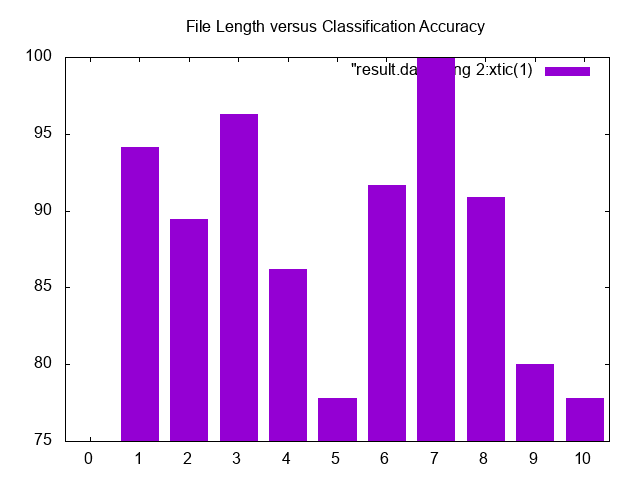
\includegraphics[scale=0.95]{d.png}};
			  \node[below=of d, node distance=0cm, yshift=1cm] {Bucket Number};
			  \node[left=of d, node distance=0cm, rotate=90, anchor=center, yshift=-1cm] {Classifiation Accuracy (\%)};
			\end{tikzpicture}
		\end{figure}

	\newpage
	\item % e
		It is easy to see that as the training data size increases, the classification accuracy also increases. But increasing the size of the training set does not necessarily solve all classification accuracy issues. At some point, it will level off. For example, it was noted that when we switched from \texttt{gen-times4} to \texttt{gen-times8}, the classification accuracy was improved only slightly.

		\begin{figure}[htb]
			\begin{tikzpicture}
			  \node[anchor=center] (e)  {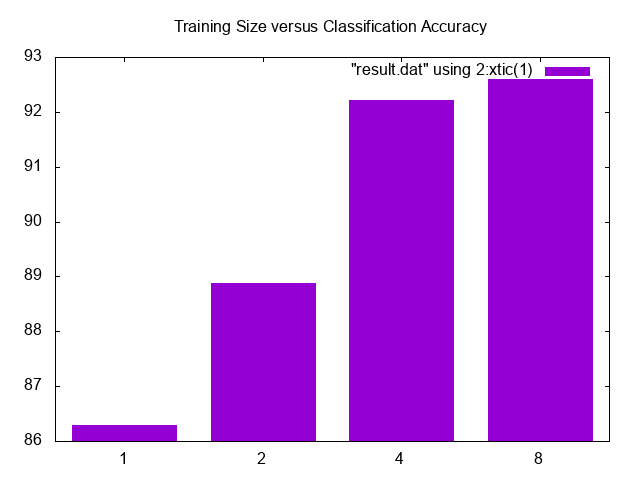
\includegraphics[scale=0.95]{e.png}};
			  \node[below=of e, node distance=0cm, yshift=1cm] {Training Size};
			  \node[left=of e, node distance=0cm, rotate=90, anchor=center, yshift=-1cm] {Classifiation Accuracy (\%)};
			\end{tikzpicture}
		\end{figure}
	\end{enumerate}

\newpage
\item % PROBLEM 4 
	\begin{enumerate}[label=(\alph*)]
	\item % a
		Let's say that we take $V =$ 19,999. 

		\begin{enumerate}[label=\roman*.]
		\item
			Using the UNIFORM estimate, if we see a word that is out of the vocabulary, we would have no choice but to assign that \textsc{oov} word a probability of 0, due to it being the 20,000th word of a vocabulary of size 19,999. 

			The reason for this is that the probabilities of all other words must sum to 1, and we cannot have a probability greater than 1.
			\begin{eqnarray*}
				\sum\limits_{i=1}^{V}{\frac{1}{V}} &=& 1 , \ \ V = \text{19,999}
			\end{eqnarray*}
			From the above equation, it is clear that we cannot assign \textsc{oov} a probability of any value other than $0$, if we are not to exceed a total probability of $1$.

			However, assigning \textsc{oov} a probability of 0 is a bad estimation, because no word should have a probability of 0, regardless of whether that word was observed in the training data.
		\item
			Using the ADDL estimate, a somewhat similar situation occurs. The ADDL probability is defined as follows.
			\begin{eqnarray*}
				\hat{p}(z \mid xy) &=& \frac{c(xyz) + \lambda}{c(xy) + \lambda V}
			\end{eqnarray*}
			Now if we were to sum the probabilities $\hat{p}(z \mid xy)$ for all $z \in \text{vocabulary}$, we would take a summation over 20,000 elements. However, if $V =$ 19,999, we would end up getting a sum that is greater than 1, which canot be true due to the laws of probability. Hence, taking $V =$ 19,999 is problematic.

		\end{enumerate}
	\item % b
		If we let $\lambda = 0$, then we are not modifying our probability at all. That is, we get the following from our probabiliy estimate.
		\begin{eqnarray*}
			\hat{p}(z \mid xy) &=& \frac{c(xyz) + \lambda}{c(xy) + \lambda V} 	\\
							   &=& \frac{c(xyz) + 0}{c(xy) + 0} 				\\
							   &=& \frac{c(xyz)}{c(xy)} 						\\
		\end{eqnarray*}
		This ends up being the naive estimate of $\hat{p}(z \mid xy)$. If no smoothing occurs, then the probabilitiy given to any trigram that did not appear in the training corpus is 0, which is not well represntative of natural language.

	\newpage
	\item % c

		\begin{enumerate}[label=\roman*.]
		\item
			First, let's think about the case when $c(xyz) = c(xyz') = 0$. \vspace{4pt}

			We see that
			\begin{eqnarray*}
				\hat{p}(z\mid xy) &=& \frac{0 + \lambda V \cdot \hat{p}(z \mid y)}{c(xy) + \lambda V}
			\end{eqnarray*}

			Then the difference between $\hat{p}(z\mid xy)$ and $\hat{p}(z' \mid xy)$ is the possible differing values of $\hat{p}(z \mid y)$ and $\hat{p}(z' \mid y)$. And we cannot guarantee that $\hat{p}(z \mid y)$ = $\hat{p}(z' \mid y)$. \vspace{4pt}

			For example, we might see neither of the phrases ``kiss the tree'' nor ``kiss the Jupiter''. However, when we backoff, it is possible that we would have seen both of the phrases ``the tree'' and ``the Jupiter'' (which are both much more common). \vspace{4pt}

			And in English, it is much more likely that the phrase ``the tree'' is more common than ``the Jupiter'', which demonstrates a case in which $\hat{p}(z \mid y) \neq \hat{p}(z' \mid y)$. \vspace{4pt}

			$\implies \hat{p}(z\mid xy) \neq \hat{p}(z' \mid xy)$. \vspace{4pt}
			
		\item
			Now let's think about the case when $c(xyz) = c(xyz') = 1$. \vspace{4pt}

			We see that
			\begin{eqnarray*}
				\hat{p}(z\mid xy) &=& \frac{1 + \lambda V \cdot \hat{p}(z \mid y)}{c(xy) + \lambda V}
			\end{eqnarray*}

			Again, the difference between $\hat{p}(z\mid xy)$ and $\hat{p}(z' \mid xy)$ is the possible differing values of $\hat{p}(z \mid y)$ and $\hat{p}(z' \mid y)$. And again, we cannot guarantee that $\hat{p}(z \mid y) = \hat{p}(z' \mid y)$. \vspace{4pt}

			For example, consider the phrases ``kick the Spongebob'' and ``kick the man'', both of which have been counted exaclty once in the training corpora. But when we backoff, it is possible that we would have seen the ``the man'' much more frequently than ``the Spongebob''. Again, this is another case in which $\hat{p}(z \mid y) \neq \hat{p}(z' \mid y)$. \vspace{4pt}

			$\implies \hat{p}(z\mid xy) \neq \hat{p}(z' \mid xy)$. \vspace{4pt}

		\end{enumerate}

	\item % d
		Again, we can write out the formula for the probability of a particular trigram using BACKOFF\_ADDL smoothing.
		\begin{eqnarray*}
			\hat{p}(z\mid xy) &=& \frac{c(xyz) + \lambda V \cdot \hat{p}(z \mid y)}{c(xy) + \lambda V}
		\end{eqnarray*}
		If we were to increase the value of $\lambda$, we would be smoothing at a greater rate. That is, we would be more heavily weighting the value of $\hat{p}(z \mid y)$ into our calculation of $\hat{p}(z \mid xy)$.

		So increasing the value of $\lambda$ would push our probabilities $\hat{p}(z \mid xy)$ closer to the probabilities $\hat{p}(z \mid y)$.

		Now note that $\hat{p}(z \mid y)$ backs off onto $\hat{p}(z)$, which is calculated using the naive estimate. Also ote that the calculation of $\hat{p}(z \mid y)$ is \textit{also} influenced by $\lambda$ (i.e. larger values of $\lambda$ push it towards $\hat{p}(z)$). So if we increase $\lambda$ to be large enough, we would eventually push the probabilities $\hat{p}(z \mid xy)$ towards $1/V$, or the uniform distribution.
	\end{enumerate}

\newpage
\item % PROBLEM 5
	\begin{enumerate}[label=(\alph*)]
	\item % a
		\texttt{IMPLEMENTATION PROBLEM}
	\item % b
		Using $\lambda^* = 0.0104$, as calculated in problem \textbf{3}(b), we can calculate the cross-entropies for the switchboard corpora and analyze the text categorization error rates for \texttt{gen}/\texttt{spam}. The following generalizations are made with the assumption that $\lambda^* = 0.0104$.
		\begin{itemize}
			\item[] \hspace{-24pt} 
				\textbf{cross-entropies for the switchboard corpora} \vspace{4pt} \\
				In problem \textbf{1}, we calculated the log-probabilities using ADDL using a $\lambda$ value of $0.01$. Because $\lambda^* = 0.0104$, we need to recalculate the log-probabilities. \vspace{4pt}

				Below contains log-probabilities using ADDL for switchboard corpora.
				\begin{lstlisting}
		-12572.8    speech/sample1
		-7544.45    speech/sample2
		-7944.22    speech/sample3
				\end{lstlisting}

				Below contains log-probabilities using BACKOFF\_ADDL for switchboard corpora.
				\begin{lstlisting}
		-10040.1    speech/sample1
		-6039.31    speech/sample2
		-6413.95    speech/sample3
				\end{lstlisting}
				
				Now to calculate the cross-entropties of the sample files, we must count the number of words in each sample file. We can do so using the following command. \vspace{4pt}

				\codebox{\$ find speech -name 'sample*' | xargs wc -w \hspace{49mm}}
				\begin{lstlisting}
		1686    speech/sample1
		978     speech/sample2
		985     speech/sample3
				\end{lstlisting}

				Then we can find the cross-entropies of each sample file by dividing the negative log-probability of each sample file by its corresponding word count. \\
				
				Below contains the cross-entropies of the switchboard corpora for each of the three samples, using ADDL and BACKOFF\_ADDL smoothing. \\

				\begin{center}\begin{tabular}{| r || c | c |}
					\hline
									& \ \ \ \ \ ADDL \ \ \ \ \ & BACKOFF\_ADDL \\
					\hline \hline
					\texttt{speech/sample1} & 7.457 & 5.955 		\\
					\texttt{speech/sample2} & 7.714 & 6.175 		\\
					\texttt{speech/sample3} & 8.065 & 6.512 		\\
					\hline
				
				\end{tabular}\end{center} \vspace{8pt}

				For each of the three speech samples, we see that switching from ADDL smoothing to BACKOFF\_ADDL smoothing decreases the cross-entropy greatly, against the training switchboard corpus.

			\item[] \hspace{-24pt} 
				\textbf{text categorization error rates for gen/spam} \vspace{4pt} \\
				Below contains output using BACKOFF\_ADDL for \texttt{gen} test files.
				\begin{lstlisting}
		337 looked more like gen_spam/train/gen (93.61%)
		23 looked more like gen_spam/train/spam (6.39%)
				\end{lstlisting}

				Below contains output using BACKOFF\_ADDL for \texttt{spam} test files.
				\begin{lstlisting}
		17 looked more like gen_spam/train/gen (9.44%)
		163 looked more like gen_spam/train/spam (90.56%)
				\end{lstlisting}
				From these outputs, we can see that the error rates using BACKOFF\_ADDL were \textit{significantly} lower than the error rates using ADDL as in \textbf{3}(c) for \texttt{spam} test files. \vspace{4pt}

				At the same time, the error rates using BACKOFF\_ADDL were \textit{slightly} higher than the error rates using ADDL as in \textbf{3}(c) for \texttt{gen} test files. \vspace{4pt}

				We can conclude that switching from ADDL to BACKOFF\_ADDL causes the error rates for classifying spam files to decrease extraordinarily, but at the cost of slightly increasing error rates for classifying genuine files. It seems to balance out the classification correctness rates a quite a bit.
		\end{itemize}
	\item % c
		\textit{Extra credit:} We were able to find $\lambda_1 = 0.1$, which works a bit better than $\lambda^*$ in a sense. By using $\lambda_1$, our classification results on test data are exactly the same, but the cross-entropies are much smaller.
	\end{enumerate}
\item % PROBLEM 6
	\begin{enumerate}[label=(\alph*)]
	\item % a
		\texttt{IMPLEMENTATION PROBLEM}
	\item % b
		\texttt{IMPLEMENTATION PROBLEM}
	\item % c
		\begin{lstlisting}
		epoch 1:   F=-3.274666
		epoch 2:   F=-3.160848
		epoch 3:   F=-3.114404
		epoch 4:   F=-3.087500
		epoch 5:   F=-3.070043
		epoch 6:   F=-3.058030
		epoch 7:   F=-3.049404
		epoch 8:   F=-3.042993
		epoch 9:   F=-3.038087
		epoch 10: F=-3.034236
		\end{lstlisting}
	\item % d
		First, we can run some experiments on the development files. Because we will need the word counts of the development files, we can get those easily using the following two commands. \vspace{4pt} \\
		\codebox{wc -w english\_spanish/dev/english/*/* \hspace{70mm}} \\
		\codebox{wc -w english\_spanish/dev/spanish/*/* \hspace{70mm}} \\

		For \texttt{english}, we have total word count of 16820. \\
		For \texttt{spanish}, we have total word count of 17069. \\

		After getting the word counts of the files, we can then calculate the negative log probabilities across each particular group of files (either \texttt{english} or \texttt{spanish}).

		To calculate the cross-entropy, we simply divide the negative log probabilities by their corresponding word counts.

		The data below contain results using development files.

		\begin{itemize}
		\item[] \hspace{-24pt} \textbf{ADDL}
			\begin{itemize}
			\item[] \hspace{-24pt} \textit{C = 1} 	 \vspace{4pt}
				\begin{center}\begin{tabular}{| r || c | c |}
				\hline
									& log-probability	& cross-entropy \\
				\hline \hline
				\texttt{english}	& $-72686.8$		& 4.321			\\
				\texttt{spanish}	& $-67682.5$		& 3.965			\\
				\hline
				
				\end{tabular}\end{center}
				
			\item[] \hspace{-24pt} \textit{C = 0.05} \vspace{4pt}
				\begin{center}\begin{tabular}{| r || c | c |}
				\hline
									& log-probability	& cross-entropy \\
				\hline \hline
				\texttt{english}	& $-70801.5$		& 4.209			\\
				\texttt{spanish}	& $-67773$			& 3.971			\\
				\hline
				
				\end{tabular}\end{center}

			\item[] \hspace{-24pt} \textit{C = 3} 	 \vspace{4pt}
				\begin{center}\begin{tabular}{| r || c | c |}
				\hline
									& log-probability	& cross-entropy \\
				\hline \hline
				\texttt{english}	& $-77439.3$		& 4.604			\\
				\texttt{spanish}	& $-72267.5$		& 4.234			\\
				\hline
				
				\end{tabular}\end{center} \vspace{8pt}

			\end{itemize} \vspace{8pt}

			Generally speaking, it would seem that increasing the value of $C$ increases the cross-entropy when using the ADDL smoothing function. 
			\vspace{8pt} \\

		\item[] \hspace{-24pt} \textbf{BACKOFF\_ADDL}
			\begin{itemize}
			\item[] \hspace{-24pt} \textit{C = 1} 	 \vspace{4pt}
				\begin{center}\begin{tabular}{| r || c | c |}
				\hline
									& log-probability	& cross-entropy \\
				\hline \hline
				\texttt{english}	& $-62616.4$		& 3.723			\\
				\texttt{spanish}	& $-61372.4$		& 3.596			\\
				\hline
				
				\end{tabular}\end{center}
				
			\item[] \hspace{-24pt} \textit{C = 0.05} \vspace{4pt}
				\begin{center}\begin{tabular}{| r || c | c |}
				\hline
									& log-probability	& cross-entropy \\
				\hline \hline
				\texttt{english}	& $-71948$			& 4.278			\\
				\texttt{spanish}	& $-72578.1$		& 4.252			\\
				\hline
				
				\end{tabular}\end{center}

			\item[] \hspace{-24pt} \textit{C = 3} 	 \vspace{4pt} \\
				\begin{center}\begin{tabular}{| r || c | c |}
				\hline
									& log-probability	& cross-entropy \\
				\hline \hline
				\texttt{english}	& $-65199.2$		& 3.876			\\
				\texttt{spanish}	& $-63375$			& 3.713			\\
				\hline
				
				\end{tabular}\end{center} \vspace{8pt}

			\end{itemize} \vspace{8pt}

			Generally speaking, it would seem that there is an optimal value of $C$ that minimizes the cross-entropy when using the BACKOFF\_ADDL. This optimal value most likely occurs somewhere in the range $(0.05, 3)$.
			\vspace{8pt} \\

		\newpage
		\item[] \hspace{-24pt} \textbf{LOGLINEAR}

			\begin{itemize}
			\item[] \hspace{-24pt} \textit{C = 1} 	 \vspace{4pt}
				\begin{center}\begin{tabular}{| r || c | c |}
				\hline
									& log-probability	& cross-entropy \\
				\hline \hline
				\texttt{english}	& $-75830.3$		& 4.443			\\
				\texttt{spanish}	& $-74669.3$		& 4.375			\\
				\hline
				
				\end{tabular}\end{center}
				
			\item[] \hspace{-24pt} \textit{C = 0.05} \vspace{4pt}
				\begin{center}\begin{tabular}{| r || c | c |}
				\hline
									& log-probability	& cross-entropy \\
				\hline \hline
				\texttt{english}	& $-75876$			& 4.445			\\
				\texttt{spanish}	& $-74640.2$		& 4.373			\\
				\hline
				
				\end{tabular}\end{center}

			\item[] \hspace{-24pt} \textit{C = 3} 	 \vspace{4pt} \\
				\begin{center}\begin{tabular}{| r || c | c |}
				\hline
									& log-probability	& cross-entropy \\
				\hline \hline
				\texttt{english}	& $-75872$			& 4.511			\\
				\texttt{spanish}	& $-74811.4$		& 4.383			\\
				\hline
				
				\end{tabular}\end{center} \vspace{8pt}

			\end{itemize} \vspace{8pt}

			Generally speaking, there does not seem to be a significant change in the cross-entropy for any $C$ in the range $[0.05, 1]$ when using the LOGLINEAR smoothing function. However, increaseing the value of $C$ past $1$ seems to increase the cross-entropy, but only slightly.
			\vspace{8pt} \\

		\end{itemize}

		After analyzing the results of changing $C$ around in relation to the effect on cross-entropy for the ADDL, BACKOFF\_ADDL, and LOGLINEAR functions, it would probably make sense to take a look at how changing $C$ around affects classification error rates of each model.

		\begin{itemize}
		\item[] \hspace{-24pt} \textbf{ADDL} \vspace{8pt}

			\begin{center}\begin{tabular}{| r || c | c | c | c |}
			\hline
							 & $C=0.0104$ & $C=0.0500$ & $C=1.0000$ & $C=3.0000$ \\
			\hline \hline
			\texttt{english} & 12.50\%    & 10.83\%	   & 8.33\%     & 6.67\%	 \\
			\texttt{spanish} & 5.04\%     & 6.72\%	   & 6.72\%     & 6.72\%	 \\
			\hline
			\end{tabular}\end{center} \vspace{8pt}

			Generally speaking, it would seem that increasing the value of $C$ decreases the classification error rate when using the ADDL smoothing function for our interval range $C \in [0.0104, 3]$.
			\vspace{8pt} \\

		\item[] \hspace{-24pt} \textbf{BACKOFF\_ADDL} \vspace{8pt}

			\begin{center}\begin{tabular}{| r || c | c | c | c |}
			\hline
							 & $C=0.0104$ & $C=0.0500$ & $C=1.0000$ & $C=3.0000$ \\
			\hline \hline
			\texttt{english} & 5.00\%     & 5.00\%	   & 5.00\%     & 7.50\%	 \\
			\texttt{spanish} & 26.89\%    & 28.57\%	   & 26.05\%    & 23.53\%	 \\
			\hline
			\end{tabular}\end{center} \vspace{8pt}

			Generally speaking, it would seem that there is an optimal value of $C$ that minimizes the classification error rate when using the BACKOFF\_ADDL. This optimal value seems to be different for \texttt{english} and \texttt{spanish}.
			\vspace{8pt} \\

		\item[] \hspace{-24pt} \textbf{LOGLINEAR} \vspace{8pt}

			\begin{center}\begin{tabular}{| r || c | c | c | c |}
			\hline
							 & $C=0.0104$ & $C=0.0500$ & $C=1.0000$ & $C=3.0000$ \\
			\hline \hline
			\texttt{english} & 21.67\%    & 21.67\%	   & 20.83 \%   & 20.00\%	 \\
			\texttt{spanish} & 41.18\%    & 41.18\%	   & 41.18 \%   & 42.02\%	 \\
			\hline
			\end{tabular}\end{center} \vspace{8pt}

			Generally speaking, all values of $C$ using the LOGLINEAR smoothing function caused high error rates for both \texttt{english} and \texttt{spanish} development files when compared with BACKOFF\_ADDL smoothing. It seems that $C = 0.0104$, on average, minimized the error rates. For the sake of time, we decided to take $C^* = 0.0104$.

			Note that these values were calculated using $\gamma_0 = 0.01$.

		\end{itemize} \vspace{8pt}

		Compared to BACKOFF\_ADDL smoothing, LOGLINEAR performed much worse. For all values of $C$ that were tested, we saw that LOGLINEAR smoothing causes higher classification error rates in both the \texttt{english} and \texttt{spanish} development files.

		After confirming this, we performed some tests with BACKOFF\_ADDL and LOGLINEAR using the \texttt{english} and \texttt{spanish} test files.

		The results are recorded below.

		\begin{itemize}
		\item[] \hspace{-24pt} \textbf{BACKOFF\_ADDL} \vspace{8pt}

			\begin{center}\begin{tabular}{| r || c | c | c | c |}
			\hline
							 & $C=0.0104$ & $C=0.0500$ & $C=1.0000$ & $C=3.0000$ \\
			\hline \hline
			\texttt{english} & 5.95\%     & 6.22\%	   & 6.76\%     & 8.11\%	 \\
			\texttt{spanish} & 23.58\%    & 24.66\%	   & 24.93\%    & 23.85\%	 \\
			\hline
			\end{tabular}\end{center} \vspace{8pt}

			Generally speaking, it would seem that there is an optimal value of $C$ that minimizes the classification error rate when using the BACKOFF\_ADDL. This optimal value seems to be different for \texttt{english} and \texttt{spanish}.
			\vspace{8pt} \\

		\item[] \hspace{-24pt} \textbf{LOGLINEAR} \vspace{8pt}

			\begin{center}\begin{tabular}{| r || c | c | c | c |}
			\hline
							 & $C=0.0104$ & $C=0.0500$ & $C=1.0000$ & $C=3.0000$ \\
			\hline \hline
			\texttt{english} & 19.73\%    & 20.00\%	   & 19.73 \%   & 19.46\%	 \\
			\texttt{spanish} & 36.04\%    & 36.04\%	   & 35.77 \%   & 36.86\%	 \\
			\hline
			\end{tabular}\end{center} \vspace{8pt}

			Generally speaking, all values of $C$ using the LOGLINEAR smoothing function caused high error rates for both \texttt{english} and \texttt{spanish} development files. It seems that $C = 0.0104$, on average, minimized the error rates. For the sake of time, we decided to take $C^* = 0.0104$.

			Note that these values were calculated using $\gamma_0 = 0.01$.

		\end{itemize} \vspace{8pt}


	\item % e
		\textit{Extra credit:} no answer.
	\item % f

		After implementing the new feature, we played around with the values of $\alpha$ for a bit and concluded that $\alpha=0.25$ generally yielded better results for classification error rates. 

		We compared the results with our old LOGLINEAR model using $C = 0.0104$.

		After running the new model, we found that the \texttt{english} test files produced an error rate of $12.70\%$, and the \texttt{spanish} test files produced an error rate of $18.73\%$. Both of these error rates are significantly lower than before the new feature was introduced.

		For \texttt{en.1K}, our program learned $\beta = 3.289$, and found a log-probability of $-152135$ for the \texttt{english} test files. With a word count of 35240, we can compute the total cross-entropy to be approximately 4.317. This is much smaller than the computed 5.197 cross-entropy of the \texttt{english} test files using BACKOFF\_ADDL.

		For \texttt{sp.1K}, our program learned $\beta = 3.522$, and found a log-probability of $-148822$ for the \texttt{spanish} test files. With a word count of 35080, we can compute the total cross-entropy to be approximately 4.242. This is much smaller than the computed 5.136 cross-entropy of the \texttt{spanish} test files using BACKOFF\_ADDL.

	\item % g
		\begin{enumerate}[label=\roman*.]
		\setcounter{enumiii}{3}
		\item % iv
			\texttt{IMPLEMENTATION PROBLEM}
		\end{enumerate}
	\end{enumerate}
\item % PROBLEM 7
	Let $w$ denote an arbitrary word. When we want to do the classification, we may want to consider the probability $P(w \text{ is spam} \mid w)$. According to Bayes's Theorem, we can write the following equation.
	\begin{eqnarray*}
		P(w \text{ is \texttt{spam}} \mid w) &=& \frac{P(w \mid w \text{ is \texttt{spam}}) \cdot P(\texttt{spam})}{P(w)} \\
	               &=& \frac{P(w \mid w \text{ is \texttt{spam}}) \cdot P(\texttt{spam})}{P(w \mid w \text{ is \texttt{spam}}) \cdot P(\texttt{spam}) + P(w \mid w \text{ is \texttt{gen}}) \cdot P(\texttt{gen})}
	\end{eqnarray*}

	$P(w \text{ is \texttt{spam}} \mid w)$ and $P(w \mid w \text{ is \texttt{gen}})$ are the probabilities generated separately from the two models we train using the \texttt{spam} and \texttt{gen} corpora.

	Now we know the following.
	\begin{eqnarray*}
		P(\texttt{spam}) &=& \frac{1}{3}
	\end{eqnarray*}
	Then the following naturally follows. 
	\begin{eqnarray*}
		P(\texttt{gen}) &=& 1 - P(\texttt{spam}) \\
			&=& \frac{2}{3}
	\end{eqnarray*}

	We can rewrite then rewrite the following.
	\begin{eqnarray*}
		P(w \text{ is \texttt{spam}} \mid w) &=& \frac{1}{1 + \frac{2P(w \mid w \text{ is \texttt{gen}})}{P(w \mid w \text{ is \texttt{spam}})}}
	\end{eqnarray*}

	By doing this, we can calculate the probability $P(w \text{ is \texttt{spam}} \mid w)$. Obviously we don't need \textit{priori} when training the model.

	In order to implement this method, we need to
	\begin{enumerate}[label=\roman*.]
		\item
			train the \texttt{gen} model and store the probabilities for all test files,
		\item
			train the \texttt{spam} model and store the probabilities for all test files,
		\item
			iterate through all $P(w \mid w \text{ is } \texttt{gen})$ and $P(w \mid w \text{ is } \texttt{spam})$, so that we can calculate $P(w \text{ is } \texttt{spam} \mid w)$.

	\end{enumerate}

	\textit{Extra credit:} We implemented this change in \texttt{problem7.py}. We tested our implementation using an extremely small value for $\lambda$ (which was \texttt{add0.00001} in our case). From this specific test, the program successfully classified approximately $33.3\%$ of the test data to be spam. That is, the result is extremely close to \textit{priori}.

\item % PROBLEM 8
	\begin{enumerate}[label=(\alph*)]
	\item
		Using Bayes’ Theorem, we can express the probability $P(\vec{w} \mid U)$ in the following equation.

		\begin{eqnarray*}
			P(\vec{w} \mid U) &=& \frac{P(U \mid \vec{w}) * P(\vec{w})}{P(U)}
		\end{eqnarray*}

		Now in order to maximize $P(\vec{w} \mid U)$, we can think about maximizing $log_2(P(\vec{w} \mid U))$. Using the rules of logarithms, note that the following statement is true.
		\begin{eqnarray*}
			log_2(P(\vec{w} \mid U)) &=& log_2(P(U \mid \vec{w})) + log_2(P(\vec{w})) - log_2(U)
		\end{eqnarray*}

		Since $log_2(U)$ remains constant for all of the possible $\vec{w}$ being considered, we can ignore the final term on the right side of the equation when maximizing $log_2(P(\vec{w} \mid U))$. \vspace{4pt}

		That is, we only need to worry about maximizing the two other terms, $log_2(P(U \mid \vec{w})) + log_2(P(\vec{w}))$. Luckiily, $log_2(P(U \mid \vec{w}))$ is provided to us in the input files. Then all we need to do is calculate $log_2(P(\vec{w}))$ using our trigram model, which will measure the extent to which it looks like English. \vspace{4pt}

		So we iterate all 9 candidates and compute $log_2(P(U \mid \vec{w})) + log_2(P(\vec{w}))$, and can thus find the candidate with the highest probability $P(\vec{w} \mid U)$.
	\item
		\texttt{IMPLEMENTATION PROBLEM}
	\item
		Some trigrams in unrestricted data are very uncommon due to the existence of words like ``uh'', ``um'', or ``huh'' intertwined inside of the sentences. \vspace{4pt}

		Therefore in order to overcome this problem we need to utilize backing off. In pratice, we set the value of $\lambda$ to be 0.01 according to our experiments on development data. We can see the overall error rates in the table below. \\

		\begin{center}\begin{tabular}{| r || c | c |}
			\hline
			\ 				&	test/easy	&	test/unrestricted 	\\
			\hline \hline
			3-gram model 	&	0.141		&	0.380				\\
			2-gram model 	&	0.159		&	0.396				\\
			1-gram model 	&	0.210		&	0.408				\\
			\hline	
		\end{tabular}\end{center}

	\end{enumerate}
\item % PROBLEM 9
	\textit{Extra credit:} no answer.
\item % PROBLEM 10
	\textit{Extra credit:}
	\begin{enumerate}[label=(\alph*)]
	\item
		We see that as $T(xy)$ approaches 1, $\hat{p}(z \mid xy)$ approaches the naive estimate. However, note that $T(xy)$ must be at least 1 for the formula not containing $\alpha$ to be applied.

		If $T(xy) = 0$, then for $\hat{p}(z \mid xy)$ to approach the naive estimate, we need to make it so that $\alpha \approx 1$. This ensures a likelihood that $\hat{p}(z \mid y)$ will back off onto the naive estimate, which will push $\hat{p}(z \mid xy)$ closer to the naive estimate.

		Thus, $\hat{p}(z \mid xy)$ approaches the naive estimate when the trigram $(x,y,z)$ is unique (i.e. there are few other words $z'$ that follow the bigram $(x,y)$), or if $\alpha \approx 1$.
	\item
		If all of the $T$ values were made to be 0, it doesn't really make sense. $T(xy)$ counts the number of words that follow $(x,y)$. But if $T(xy) =0$ for all $(x,y) \in \text{corpus}$, then it means that there are no trigrams in the entire corpus!

		However, let's assume that we redefine $T$ and force them to be 0 anyway. If all of the $T$ values were made to be 0, then each discounted probability would approach the naive estimate. This answer naturally follows from the answer above.


	\end{enumerate}
\item % PROBLEM 11
	\textit{Extra credit:} no answer.

\end{enumerate}

\end{document}
